% Source: graduate-coursework/Sp26/CSCE763/Course_Assignments/HW2/HW2_CSCE_763_solutions.tex

\documentclass[border=4pt]{standalone}
\usepackage{amsmath}
\usepackage{amssymb}
\usepackage{graphicx}
\usepackage{tikz}
\usepackage{xcolor}
\usetikzlibrary{shapes.geometric, arrows.meta, positioning, patterns, calc}

\definecolor{USC_Garnet}{HTML}{73000A}
\definecolor{USC_Sandstorm}{HTML}{FFF2E3}
\definecolor{USC_Black90}{HTML}{363636}
\definecolor{USC_Black70}{HTML}{5C5C5C}
\definecolor{USC_Black50}{HTML}{A2A2A2}
\definecolor{USC_Black10}{HTML}{ECECEC}
\definecolor{USC_Honeycomb}{HTML}{65780B}
\definecolor{USC_Atlantic}{HTML}{466A9F}
\definecolor{USC_Congaree}{HTML}{1F414D}
\definecolor{USC_Rose}{HTML}{CC2E40}
\definecolor{USC_Grass}{HTML}{CED318}
\definecolor{USC_Horseshoe}{HTML}{65780B}
\definecolor{outputbg}{RGB}{245,245,245}

\begin{document}
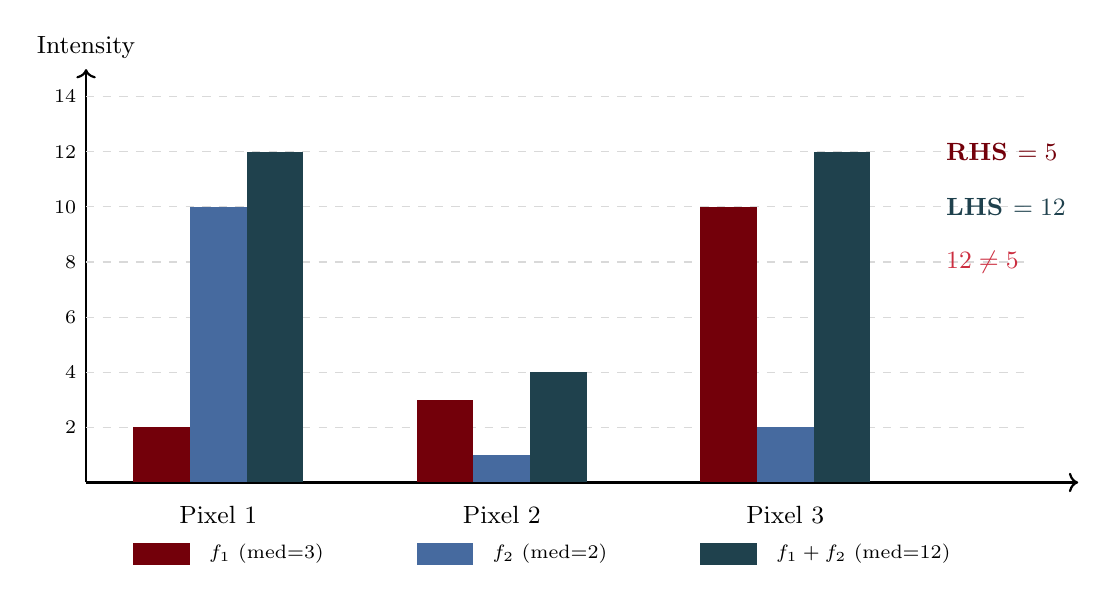
\begin{tikzpicture}[yscale=0.35, xscale=1.2]
% Axes
\draw[->, thick] (0,0) -- (10.5,0);
\draw[->, thick] (0,0) -- (0,15) node[above, font=\small] {Intensity};
% Y gridlines
\foreach \y in {2,4,6,8,10,12,14} {
  \draw[dashed, gray!30] (0,\y) -- (10,\y);
  \node[left, font=\scriptsize] at (0,\y) {\y};
}
% Bar groups: 3 pixels, 3 bars each
% Pixel 1
\fill[USC_Garnet] (0.5,0) rectangle (1.1,2);
\fill[USC_Atlantic] (1.1,0) rectangle (1.7,10);
\fill[USC_Congaree] (1.7,0) rectangle (2.3,12);
\node[below, font=\small] at (1.4,-0.5) {Pixel 1};
% Pixel 2
\fill[USC_Garnet] (3.5,0) rectangle (4.1,3);
\fill[USC_Atlantic] (4.1,0) rectangle (4.7,1);
\fill[USC_Congaree] (4.7,0) rectangle (5.3,4);
\node[below, font=\small] at (4.4,-0.5) {Pixel 2};
% Pixel 3
\fill[USC_Garnet] (6.5,0) rectangle (7.1,10);
\fill[USC_Atlantic] (7.1,0) rectangle (7.7,2);
\fill[USC_Congaree] (7.7,0) rectangle (8.3,12);
\node[below, font=\small] at (7.4,-0.5) {Pixel 3};
% Legend
\fill[USC_Garnet] (0.5,-3) rectangle (1.1,-2.2); \node[right, font=\scriptsize] at (1.2,-2.6) {$f_1$ (med$=$3)};
\fill[USC_Atlantic] (3.5,-3) rectangle (4.1,-2.2); \node[right, font=\scriptsize] at (4.2,-2.6) {$f_2$ (med$=$2)};
\fill[USC_Congaree] (6.5,-3) rectangle (7.1,-2.2); \node[right, font=\scriptsize] at (7.2,-2.6) {$f_1+f_2$ (med$=$12)};
% Annotations
\node[anchor=west, text=USC_Garnet, font=\small\bfseries] at (9,12) {RHS $= 5$};
\node[anchor=west, text=USC_Congaree, font=\small\bfseries] at (9,10) {LHS $= 12$};
\node[anchor=west, text=USC_Rose, font=\small\bfseries] at (9,8) {$12 \neq 5$};
\end{tikzpicture}
\end{document}
